\section{Architecture}
\label{architecture}

We present the BlogForever crawler system architecture which implements 
the proposed algorithms for weblog data extraction via the generation 
of extraction rules. We describe the system architecture and discuss 
the software tools and techniques we used, such as the enrichment of the 
Scrapy framework for our specific usage and the integration of a headless 
web browser into the harvesting process to achieve content extraction 
from webpages which use JavaScript to display content. Following, 
we focus on the scalability design and distributed architecture of our 
system. Finally, we present our provisions for interoperability using 
established open standards which increases the value and reusability 
of the proposed system in many contexts. 

%%%%%%%%%%%%%%%%%%%%%%%%%
\subsection{System and workflow}

The BlogForever crawler is a Python\footnote{\label{python}\url{http://www.python.org/}} 
application which is based on  Scrapy, an open-source framework for web crawling. 
Scrapy provides an elegant and modular architecture illustrated 
in Fig. \ref{scrapyarchitecture}. Several components can be plugged into 
the Scrapy core infrastructure. Following, we present each part of the 
architecture and our own contributions:

\begin{itemize}
\item 
\emph{Spiders} define how a target website is scraped, including how to 
perform the crawl (i.e. follow links). The BlogForever crawer implementation
includes two new types of spiders: \emph{NewCrawl} and \emph{UpdateCrawl},
which implement the logic to respectively crawl a new blog and get updates
from a previously crawled blog.
\item 
\emph{Item Pipeline} defines the processing of extracted data from 
the spiders through several components that are executed sequentially. 
The BlogForever crawler implementation includes a new item pipeline 
which orchestrates all aspects of crawling. More specifically the 
BlogForever pipeline is defined as follows:
  \begin{enumerate}
  \item JavaScript rendering,
  \item Extract content,
  \item Extract comments,
  \item Download multimedia files,
  \item Prepare Archival Information Packages (APIs) to propagate 
the results to potential back-ends.
  \end{enumerate}
\item 
\emph{Downloader Middlewares} is a framework of hooks into Scrapy’s 
request/response processing and altering Scrapy’s requests and responses. 
\item 
\emph{Spider Middlewares} is a framework of hooks into Scrapy’s spider 
processing mechanism.
\end{itemize}

\begin{figure}[t]
\capstart
\centering
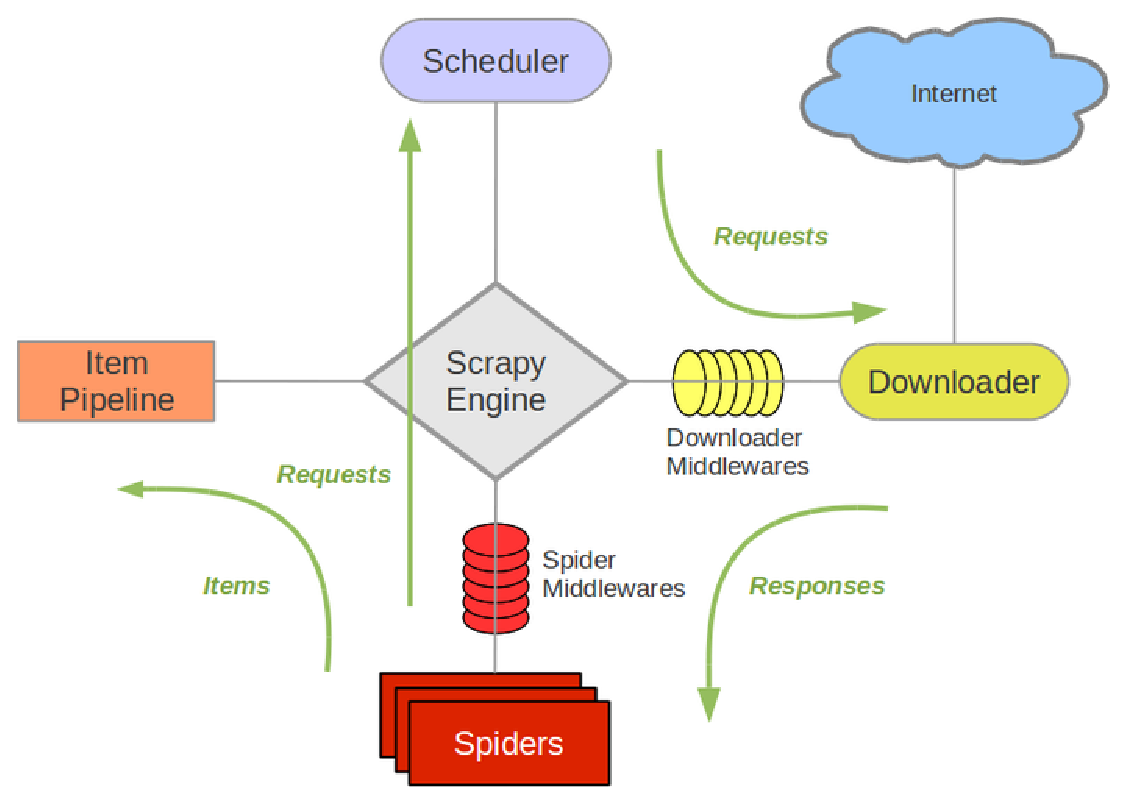
\includegraphics[width=\textwidth]{./img/scrapy_architecture.eps}
\caption{Overview of the crawler architecture. (Credit: Pablo Hoffman, Daniel Graña, Scrapy)}
\label{scrapyarchitecture}
\end{figure}

The system architecture providers great modularity. This is illustrated 
clearly in our work with the following
example:

\begin{itemize}
\item 
If it is necessary to disable JavaScript rendering or plugging in an 
alternative back-end can be done by editing a single line of code. 
\item The features to extract comments and download multimedia files 
were implemented after creating the initial logic to extract content 
and were added as extra steps in the pipeline.
\item The requirement to implement interoperability provisions later 
presented in section \ref{interop} was easily covered with the implementation 
of an extra middleware plugin which was invoked from the main crawler 
architecture. No further modifications were necessary in the code.
\end{itemize}


In the remaining parts of this section, we elaborate our work on each 
specific part of the crawler system.

%%%%%%%%%%%%%%%%%%%%%%%%%%%%%%%%%
\subsection{JavaScript rendering}

JavaScript is a widely used language for client-side scripting. 
While some applications simply use it for aesthetics, an increasing 
number of websites use JavaScript to download and display content. 
In such cases, traditional HTML based crawlers do not see web pages 
as they are presented to a human visitor by a web browser, and might 
therefore be obsolete for data extraction.

In our experiments whilst crawling the blogosphere, we encountered 
several blogs where crawled data was incomplete because of the lack 
of JavaScript interpretation. The most frequent cases were blogs using 
the Disqus\footnote{\url{http://disqus.com/websites}} and 
LiveFyre\footnote{\url{http://web.livefyre.com}} comment hosting services. 
For webmasters, these tools are very handy because the entire comments 
infrastructure is externalized and their setup essentially comes down 
to including a JavaScript snippet in each target page. Both of these 
services heavily rely on JavaScript to download and display the comments, 
even providing functionalities such as real-time updates for edits and 
newly written comments. Less commonly, some blogs are fully rendered 
using JavaScript. When loading such websites, the web browser will not 
receive the page content as an HTML document, but will instead have 
to execute JavaScript code to download and display the page content. 
The Blogger platform provides the \emph{Dynamic Views} as a default 
template, which uses this mechanism~\cite{antinharasymiv2011}.

To support blogs with JavaScript-generated content, we embed a full web 
browser into the crawler. After considering multiple options, we opted 
for PhantomJS\footnote{\url{http://phantomjs.org}}, a headless web 
browser with great performance and scripting capabilities. The JavaScript 
rendering is the very first step of web page processing. Therefore, 
extracting blog post articles, comments or multimedia files works equally 
well on blogs with JavaScript-generated content and on traditional 
HTML-only blogs.

When the number of comments on a page exceeds a certain threshold, both 
Disqus and LiveFyre will only load the most recent ones and the stream 
of comments will end with a \emph{Show More Comments} button. As part of 
the page loading process, we instruct PhantomJS to repeatedly click on 
these buttons until all comments are loaded. Paths to Disqus and LiveFyre 
\emph{Show More} buttons are manually obtained. They constitute the 
only non-generic elements of our extraction stack which require human 
intervention to maintain and extend to other commenting platforms.

%%%%%%%%%%%%%%%%%%%%%%%%%%%%%
\subsection{Content extraction}\label{enrichingscrapy}

In order to identify web pages as blog posts, our implementation enriches 
Scrapy with two components to narrow the extraction process down to the 
subsets of pages which are blog posts: \emph{blog post identification} 
and \emph{download priority heuristic}.

Given a URL entry point to a website, the default Scrapy behaviour 
traverses all the pages of the same domain in a \emph{last-in-first-out} 
manner. The \emph{blog post identification} function is able to identify 
whether an URL points to a blog post or not. Internally, for each blog, 
this function uses a regular expression constructed from the blog post 
URLs found in the web feed. This simple approach requires that blogs use 
the same URL pattern for all their posts (or false negatives will occur) 
which has to be distinct for pages that are not posts (or false positives 
will occur). In practice, this assumption holds for all blog platforms 
we encountered and seems to be a common practice among web developers.

In order to efficiently deal with blogs that have a large number of 
pages which are not posts, the \emph{blog post identification} mechanism 
is not sufficient. Indeed, after all pages identified as blog posts 
are processed, the crawler needs to download all other pages to search 
for additional blog posts. To replace the naive \emph{random walk}, 
\emph{depth first search} or \emph{breadth first search} web site 
traversals, we use a priority queue where priorities for new URLs are 
determined by a machine learning system. This mechanism has shown 
to be mandatory for blogs hosted on a single domain alongside large 
number of other types of web pages, such as those in forums or wikis.

The idea is to give high priority to URLs which are believed to 
point to pages with links to blog posts. These predictions are 
done using an active \emph{Distance-Weighted $k$-Nearest-Neighbour} 
classifier~\cite{dudani1976}. Let $L(u)$ be the number of links to blog 
posts contained in a page with URL $u$. Whenever a page is downloaded, 
its URL $u$ and $L(u)$ are given to the machine learning system as 
training data. When the crawler encounters a new URL $v$, it will ask the 
machine learning system for an estimation of $L(v)$, and use this value 
as the download priority of $v$. $L(v)$ is estimated by calculating a 
weighted average of the values of the $k$ URLs most similar to $v$.

%%%%%%%%%%%%%%%%%%%%%%%%%%%%%
\subsection{The BlogForever metadata schema for interoperability}
\label{interop}

One of the key BlogForever project goals is interoperability with third 
party platforms. The original BlogForever crawler was intended to
insert blog data directly to the BlogForever repository component but
later the architecture was reworked to make it possible to use
other storage and archiving systems as well. 
To achieve this goal, we implement a special interoperability middleware 
for the spider to produce Archival Information Packages (AIPs) from 
harvested blog content. The AIPs can be used by any software platform 
which complies with the OAIS reference model~\cite{lavoie2000meeting}. 
It must be noted also that this is the first time weblog content is 
encoded in this way.

The AIPs consist of XML files structured using the 
METS~\cite{cantara2005mets} standard for encoding metadata and 
content. METS is widely adopted and supported by all popular digital 
library systems. In addition, the blog content attributes which 
are included in the METS XML packages are encoded using the MARCXML
Schema\cite{marc2003official}. The reason for the selection of MARCXML 
is the wide adoption of the standard, its flexibility and extensibility, 
as well as previous experience with the Invenio digital library
system\footnote{\url{http://invenio-software.org/}} which is also based
on MARCXML.

There are three kinds of entities which can be included in an AIP: 
Blog, Entry and Comment. The content extracted from weblogs is mapped 
to the relevant entities using the following rule: If an attribute is 
already defined in MARC for other content types use the same MARC code 
for blogs. If an attribute is totally new, an unused MARC 9xx tag is 
chosen to represent it, composing therefore the BlogForever metadata 
schema~\cite{llopis2012d4}. Following, we present the BlogForever 
metadata schema for Blog, Post, Page and Comment entities in Tables 
\ref{table:blog-record-attributes}, 
\ref{table:post-page-shared-attributes} and 
\ref{table:comment-attributes}.

\begin{table}
\tbl{Blog record attributes - MARC 21 representations mapping.}
{\begin{tabular}{@{}ll@{}} \toprule
\textbf{Blog attribute} & \textbf{MARC 21 representation} \\ \hline
title & 245 \$a \\
subtitle & 245 \$b \\
URI & 520 \$u\\
aliases & 100 \$g \\
status\_code & 952 \$a\\
language & 041 \$a\\
encoding & 532\\
sitemap\_uri & 520\\
platform & 781 \$a\\
platform\_version & 781 \$b\\
webmaster & 955 \$a\\
hosting\_ip & 956 \$a\\
location\_city & 270 \$d\\
location\_country & 270 \$b\\
last\_activity\_date & 954 \$a\\
post\_frequency & 954 \$b\\
update\_frequency & 954 \$c\\
copyright & 542\\
ownership\_rights & 542\\
distribution\_rights & 542\\
access\_rights & 542\\
license & 542 \$f\\ \hline
\end{tabular}}
\label{table:blog-record-attributes}
\end{table}

\begin{table}
\tbl{Blog record attributes - MARC 21 representations mapping.}
{\begin{tabular}{@{}ll@{}} \toprule
\textbf{Post and page attribute} & \textbf{MARC 21 representation} \\ \hline
title & 245 \$a \\
subtitle & 245 \$b \\
full\_content & 520 \$a \\
full\_content\_format & 520 \$b \\
author & 100 \$a \\
URI & 520 \$u \\
aliases & 100 \$g \\
alt\_identifier (UR) & 0247 \$a \\
date\_created & 269 \$c\\
date\_modified & 260 \$m \\
version & 950 \$a \\
status\_code & 952 \$a \\
response\_code & 952 \$b \\
geo\_longitude & 342 \$g \\
geo\_latitude & 342 \$h \\
access\_restriction & 506 \\
has\_reply & 788 \$a \\
last\_reply\_date & 788 \$c \\
num\_of\_replies & 788 \$b \\
child\_of & 760 \$o \$4 \$w\\
\hline
\end{tabular}}
\label{table:post-page-shared-attributes}
\end{table}

\begin{table}
\tbl{Comment record attributes - MARC tags mapping.}
{\begin{tabular}{@{}ll@{}} \toprule
\textbf{Comment attribute} & \textbf{MARC 21 representation} \\ \hline
subject & 245 \$a\\
author & 100 \$a \\
full\_content & 520 \$a \\
full\_content\_format & 520 \$b \\
URI & 520 \$u\\
status & 952 \$a\\
date\_added & 269 \$c\\
date\_modified & 269 \$m\\
addressed\_to\_URI & 789 \$u\\
%& \textit{timezone} & \\
%& \textit{format} & \\
%& comment\_type (UR) & \\
%& source\_URI (UR) & \\
%& source\_name (UR) & \\
geo\_longitude & 342 \$g \\
geo\_latitude & 342 \$h \\
has\_reply & 788 \$a \\
num\_replies & 788 \$b\\
is\_child\_of\_post & 773 \$o \$4 \$w\\
is\_child\_of\_comment & 773 \$o \$4 \$w\\ \hline
\end{tabular}}
\label{table:comment-attributes}
\end{table}

%%%%%%%%%%%%%%%%%%%%%%%%
\subsection{Distributed architecture and scalability}
\label{scalability}

One of the problems of web crawling is the large amount 
of input which need to be processed. To address this issue, 
it is crucial to build every layer of the system with scalability in 
mind~\cite{thereactivemanifesto2013}. 

The BlogForever Crawler, and in particular the two core procedures 
\emph{NewCrawl} and \emph{UpdateCrawl}, are designed to be usable as 
part of an event-driven, scalable and fault-resilient distributed system. 
Heading in this direction, we made the key design choice to have 
both \emph{NewCrawl} and \emph{UpdateCrawl} as stateless components. 
From a high-level point of view, these two components are \emph{purely functional}:
%
\begin{eqnarray*}
NewCrawl:    &~ URL \rightarrow \mathcal{P}(RECORD) \\
UpdateCrawl: &~ URL \times DATE \rightarrow \mathcal{P}(RECORD)
\end{eqnarray*}
%
where $URL$, $DATE$ and $RECORD$ are respectively the set of all URLs, 
dates and records, and $\mathcal{P}$ designates the power set operator. 
By delegating all shared mutable state to the back-end system, 
web crawler instances can be added, removed and used interchangeably.

To implement a distributed crawler architecture, we choose to use 
Scrapyd\footnote{\url{http://scrapyd.readthedocs.org/en/latest/}}, 
an application for deploying and running Scrapy spiders. 
The process is quite straightforward:

\begin{enumerate}
\item 
Deploy the BlogForever crawler in any number of servers according 
to requirements. Using the Scrapyd component which is run as a system 
daemon, each crawler is listening for requests to run crawling tasks 
and spawn a process for each new command.
\item 
Implement a small control program that reads the list of target weblogs 
which need to be crawled and issue commands in a round-robin fashion 
using the Scrapyd JSON 
API\footnote{\url{http://scrapyd.readthedocs.org/en/latest/api.html}}. 
\item 
All crawlers share a common storage service where they save the crawling 
results. 
\end{enumerate}

